

\section{Beispiel}

\begin{frame}{Aufgabe}
	\begin{itemize}
		\item Webserver für Most Useless Machine Ever!
	\end{itemize}
	\begin{center}
		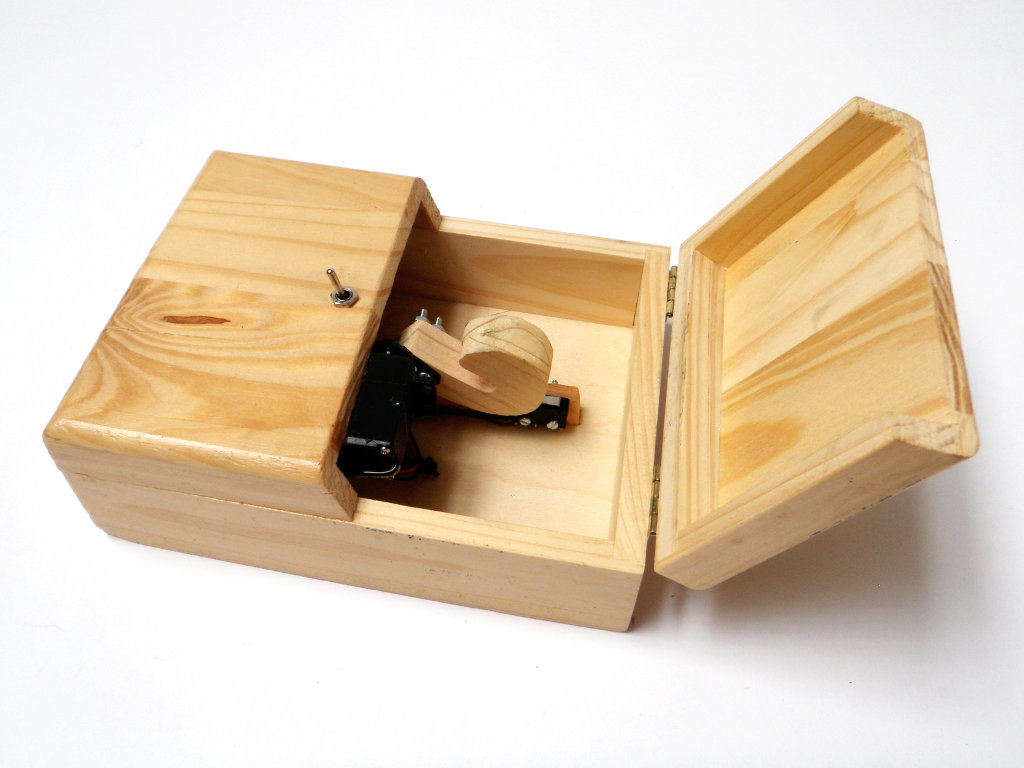
\includegraphics[width=0.75\textwidth]{res/mume.jpg}
		\cite{mumePic}
	\end{center}
\end{frame}

\begin{frame}{System}
	\begin{itemize}
		\item uC oder GNU/Linux?
		\item Gegenüber einem uC wie Arduino bringt GNU/Linux
		\begin{itemize}
			\item Hardware-Treiber
			\item Protokolle
			\item Tools
			\item erhöhte Komplexität
		\end{itemize}
	\end{itemize}
\end{frame}

\begin{frame}{Hardware}
	\begin{itemize}
		\item Eval-/Bastelboards (Raspi, BeagleBone)
		\item Consumer Hardware (Router, Media-Center, \ldots)
		\item Profesionelle Boards
		\item[$\rightarrow$] BeagleBone Green
		\begin{itemize}
			\item Netzwerk
			\item USB
			\item Yocto Supported
			\item viele Anshlüsse
			\item USB Powered
			\item kein Display Anschluss
			\item bereits Erfahrung
		\end{itemize}
	\end{itemize}
\end{frame}

\begin{frame}{Developer Image}
	\begin{itemize}
		\item Wie kriegen wir ein Linux drauf?
		\item[$\rightarrow$] Yocto
	\end{itemize}
\end{frame}

\begin{frame}{SDK}
	\begin{itemize}
		\item Wie können wir Software dafür kompilieren?
		\item[$\rightarrow$] Yocto SDK
		\begin{itemize}
			\item cross compiler
			\item root file system
		\end{itemize}
	\end{itemize}
\end{frame}

\begin{frame}{Treiber}
	\begin{itemize}
		\item wie können wir die Hardware ansteuern?
		\item[$\rightarrow$] Linux Treiber
		\begin{itemize}
			\item GPIO
			\item PWM
			\item sysfs
			\item Device-Tree
		\end{itemize}
	\end{itemize}
\end{frame}

\begin{frame}{MUME Service}
	\begin{itemize}
		\item wie können wir mit dem Treiber kommunizieren?
		\item[$\rightarrow$] sysfs / D-Bus
		\begin{itemize}
			\item Service der den Treiber weiter abstrahiert
		\end{itemize}
	\end{itemize}
\end{frame}

\begin{frame}{GUI}
	\begin{itemize}
		\item Koennen wir via Browser auf das System zugreifen?
		\item[$\rightarrow$] gui
		\begin{itemize}
			\item nginx
			\item fastcgi
			\item gui
			\item D-Bus
		\end{itemize}
	\end{itemize}
\end{frame}

\begin{frame}{Service Manager}
	\begin{itemize}
		\item Wie starten und managen wir die Services?
		\item[$\rightarrow$] systemd
		\begin{itemize}
			\item service files schreiben
			\item fastcgi
			\item gui
			\item D-Bus
		\end{itemize}
	\end{itemize}
\end{frame}

\begin{frame}{Produktiv Image}
	\begin{itemize}
		\item Wie können wir die Firmware verteilen?
		\item[$\rightarrow$] Yocto
	\end{itemize}
\end{frame}







\begin{frame}{system}
	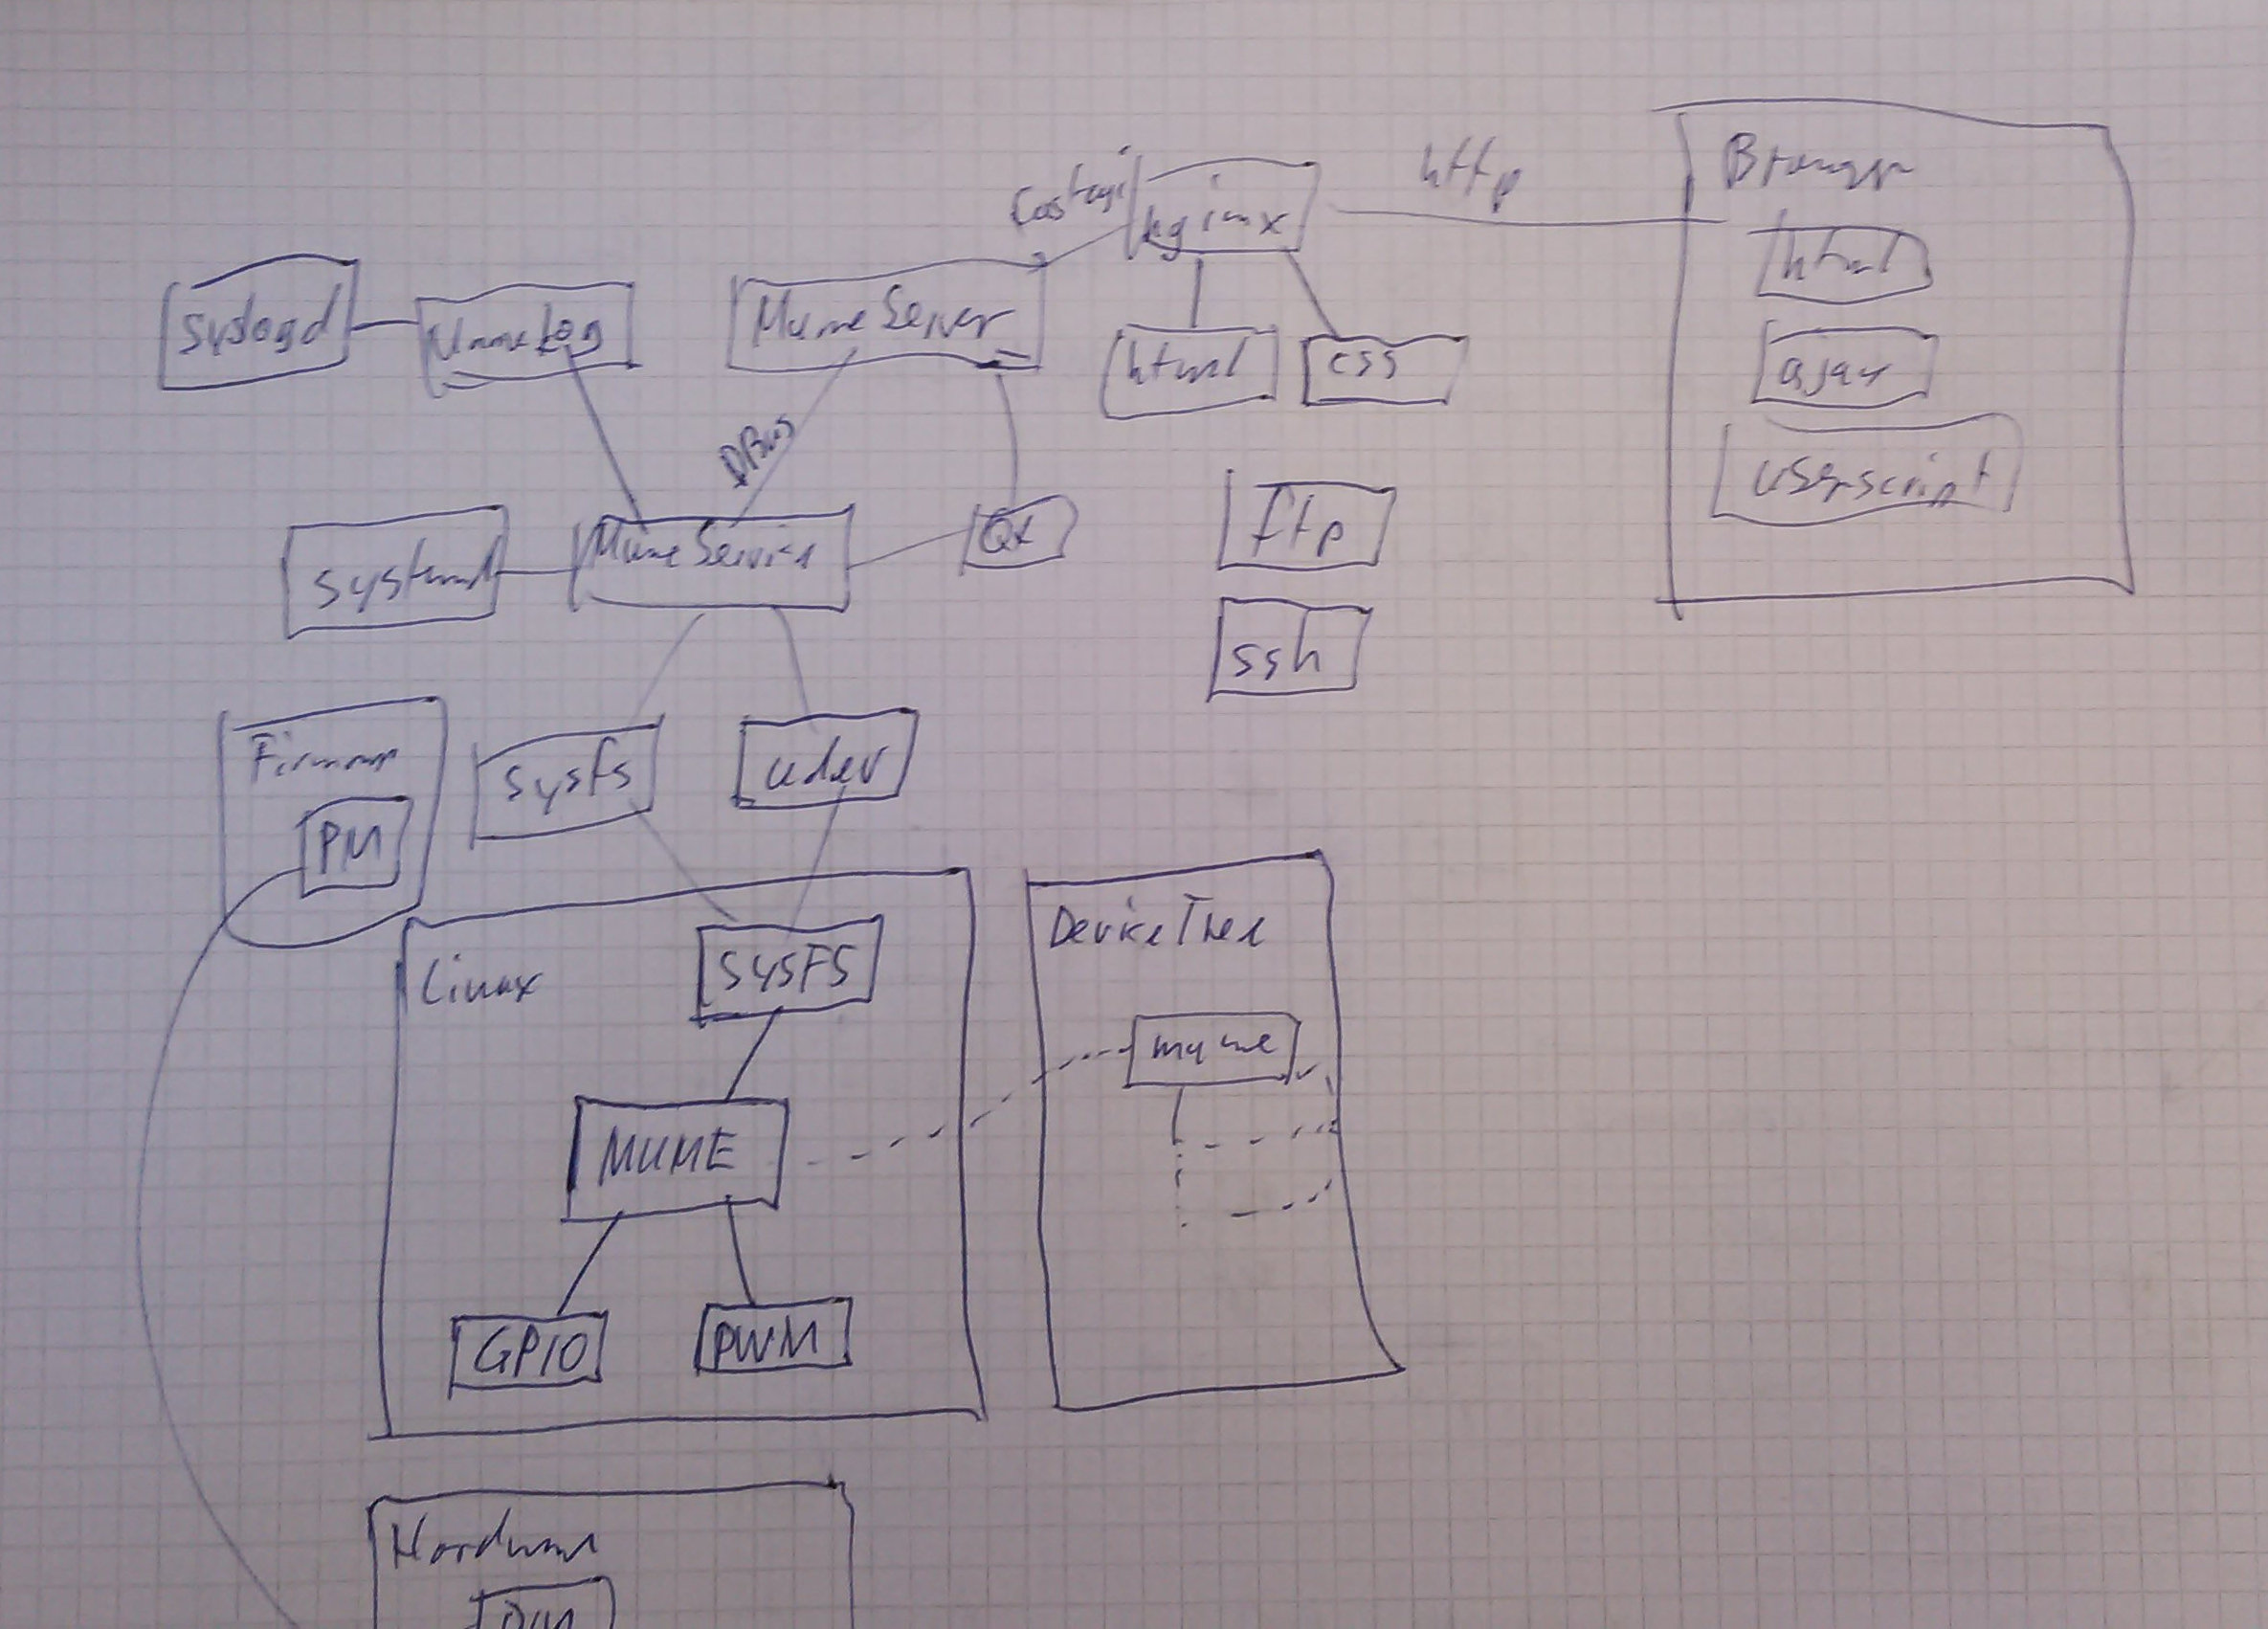
\includegraphics[width=\textwidth]{res/system.jpg}
\end{frame}

\begin{frame}{Linux}
	\begin{itemize}
		\item Sammlung von Subsystemen, abstraktionenen
		\item i2c
		\item spi
		\item iio
		\item fbtft
		\item gpio
		\item led
	\end{itemize}
\end{frame}

\begin{frame}{eigener Treiber}
	Beispiel ``Most Usless Machine Ever''
\end{frame}

\begin{frame}{Applikationen}
	Siehe System
	\begin{itemize}
		\item Embedded System besteht meist aus mehreren Prozessen $\rightarrow$ Microservices
		\item Webserver, Prozessueberwachung, SSH, FTP, UI
		\item gutes IPC system (z.B. kdbus)
		\item eigener Service
		\begin{itemize}
			\item reaktiv, event-getriggert
			\item Qt gut geeignet
			\item andere Frameworks moeglich
			\item auch ohne Framework moeglich
		\end{itemize}
	\end{itemize}
\end{frame}

\begin{frame}{Webserver}
\end{frame}